\section{Evidence that Prophet does not solve its objective}
\label{sec:evidence}

Each piece of evidence below answers a different objection. A gap in the
objective could be a difference in what is being fitted rather than how; a
difference in where two optimizers stop could reflect non-uniqueness rather than
non-convergence; and a failure could be an artefact of one algorithm rather than
of the objective. The controls are chosen to rule each of those out in turn.

\subsection{The optimum, under Prophet's own density}
\label{sec:evidence:lp}

We score both solutions with Stan's own log density, evaluated through
\code{CmdStanModel.log_prob} on Prophet's compiled model, fitting both on
Prophet's own changepoint locations so that only the optimizer differs. On the
Peyton Manning series in Prophet's default configuration the corrected optimum
is higher at every length measured, by \LpMarginShort{} nats at $T = 300$,
\LpMarginMid{} at $T = 1000$ and \LpMarginLong{} at $T = 2905$.

As a share of the posterior the margin falls by a factor of \LpDecline{} across
that range, from \LpPercentShort\% to \LpPercentLong\%. The margin itself does not
decline, and it depends on the width of the model as much as its length: with yearly
seasonality alone the margin at $T = 2905$ is \MarginYearlyLong{} nats rather than
\LpMarginLong.

\begin{figure}[t]
  \centering
  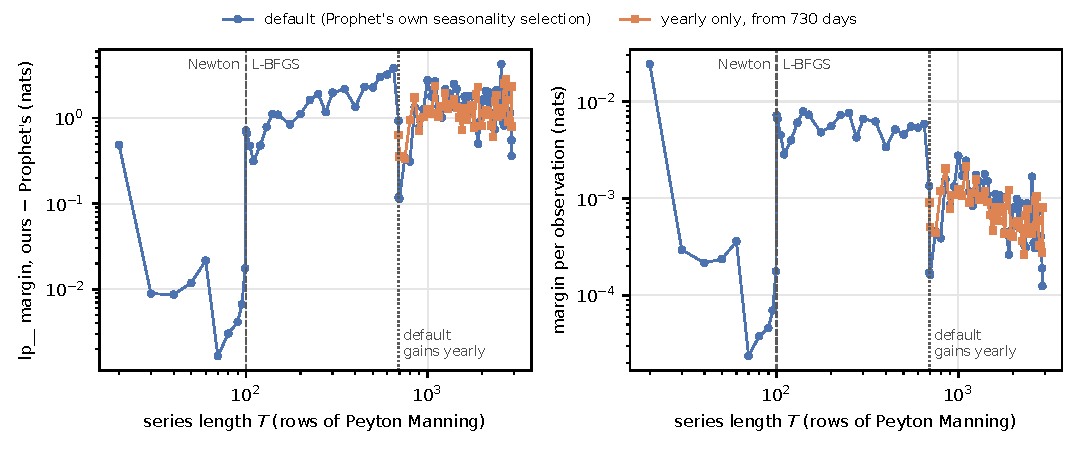
\includegraphics[width=\textwidth]{figures/margin_vs_length}
  \caption{The $\lp$ margin of the corrected optimum over Prophet's, under Prophet's
    own density, fitted on the first $T$ rows of the Peyton Manning series:
    absolute (left) and as a share of Prophet's $\lp$ (right), on logarithmic
    axes. Higher means Prophet stopped further from the optimum. Blue is Prophet's
    default seasonality selection, which adds yearly seasonality once the history
    spans 730 days, at $T = \MarginYearlyFrom$ (dotted); orange forces yearly
    seasonality alone and starts there. Left of the dashed line Prophet, and this
    implementation, run Newton's method; right of it, L-BFGS. Below $T = 33$ Prophet
    places fewer than 25 changepoints.}
  \label{fig:margin}
\end{figure}

\Cref{fig:margin} measures the margin on a finer grid: \MarginCells{} fits, at
\MarginLengths{} lengths from $T = 20$ to $2905$ in the default configuration and at
those from $T = \MarginYearlyFrom$ with yearly seasonality alone. The margin is
positive in every one of them. Its absolute size has no trend in $T$: wherever
Prophet runs L-BFGS it moves between \MarginLbfgsMin{} and \MarginLbfgsMax{} nats from
one length to the next, with a median of \MarginLbfgsMedian, while $\lp$ itself grows
roughly in proportion to $T$, so the fall of the relative margin is the growth of
its denominator. Two steps do coincide with a change in the problem or in the
solver. Where the default model gains yearly seasonality the margin falls from
\MarginBeforeYearly{} to \MarginAfterYearly{} nats. And between $T = 99$ and
$T = 100$ the data gain one observation, Prophet's solver changes from Newton to
L-BFGS, and the margin rises from \MarginAtNinetyNine{} to \MarginAtHundred{} nats.
Across the Newton range the median margin is \MarginNewtonMedian{} nats, against
\MarginLbfgsMedian{} across the L-BFGS one, so the size of the gap at short lengths is
largely a statement about which method Prophet ran.

We state the direction, which holds in every configuration measured, and claim no
mechanism for the size. It also holds across the census of \cref{sec:consequences}:
fitted on each series' full length, the corrected optimum scores higher on
\KktLpWins{} of the \KktSeries{} series, by a median of \KktLpMedian{} nats and never
by less than \KktLpMin.

Nor is the margin a matter of Prophet's stopping tolerances. Stan's L-BFGS has five
tests besides its budget of iterations, and with every one set to machine precision or
below it runs on until an iteration makes no progress or its line search fails. On the
full series that takes it from iteration \TolDefaultIterLong{} to
\TolFiveIterLong{}, and it still ends \TolFiveShortLong{} nats short of the optimum
(\TolDefaultShortLong{} at the defaults); at $T = 300$ and $1000$ it ends
\TolFiveShortShort{} and \TolFiveShortMid{} nats short, against \TolDefaultShortShort{}
and \TolDefaultShortMid. With yearly seasonality alone at $T = 2905$ it runs
\TolFiveIterYearly{} iterations instead of \TolDefaultIterYearly{} and closes the gap
from \TolDefaultShortYearly{} to \TolFiveShortYearly{} nats, and no further. These runs
call Stan directly, because where the line search fails Prophet cannot report the
result: it treats the failure as an abnormal exit and retries with Newton, passing the
tolerances on, and cmdstanpy rejects them for Newton, so the fit raises an error.

\subsection{First-order optimality}
\label{sec:evidence:kkt}

A margin in $\lp$ compares two points; a first-order certificate grades each on
its own. Write \eqref{eq:objective} as a smooth part $s$ plus
$\tau^{-1}\sum_j\lvert\delta_j\rvert$ and hold $\sigma$ at the point's own value. The
point is a minimiser if and only if $0$ lies in the subdifferential there:
$\partial s/\partial x = 0$ for $x$ among $k$, $m$ and $\beta$;
$\partial s/\partial\delta_j + \operatorname{sign}(\delta_j)/\tau = 0$ wherever
$\delta_j \ne 0$; and $\lvert\partial s/\partial\delta_j\rvert \le 1/\tau$ wherever
$\delta_j = 0$. The norm of the subdifferential's minimum-norm element measures how far
a point is from meeting them. The ``if'' is the convexity of \cref{sec:model}, which
holds in Prophet's default configuration once $\sigma$ is fixed. Fixing it costs the
argument nothing in the direction that matters: a point optimal for the full problem
is stationary in the other coordinates at its own $\sigma$, so a residual bounded
away from zero proves it is not optimal, with $\sigma$ free or not.

The gradient is Stan's, of Prophet's compiled density, through
\code{CmdStanModel.log_prob}, so neither implementation grades itself; at the
reformulation's solution it agrees with this implementation's hand-derived gradient
to $10^{-7}$. Prophet's point is read at full precision. CmdStan writes the optimum
with eight significant digits unless asked otherwise, and on \KktRoundingSeries{}
census series drawn at random that rounding alone moves Prophet's residual by up to
\KktRoundingMax, against a residual of at least \KktRoundingResidualMin{} on every one of
them.

Each of the \KktSeries{} series of the census of \cref{sec:consequences} is fitted on
its full length in Prophet's default configuration. Prophet's residual has a median
of \KktProphetStrict{}, against \KktOursMedian{} for the reformulation. The prediction
was a residual of order $1/\tau = 20$ wherever Prophet leaves a rate small but not
zero, and that is where it lies: on \KktStrictAtRate\% of series the largest violation
is a changepoint rate, of median magnitude $\KktKinkRate$, which has to balance the
prior's full slope $1/\tau$ and does not.

The obvious objection is that such a rate is zero in all but name. The relaxed
residual grants that to every rate at once, holding each $\delta_j$ only to the
condition for $\delta_j = 0$. Since $\operatorname{sign}(\delta_j)/\tau$ is an endpoint
of $[-1/\tau, 1/\tau]$, the relaxed residual is never larger than the strict one,
needs no threshold for what counts as zero, and is still a lower bound on the distance
from $0$ to the subdifferential at the point. Prophet's has a median of
\KktProphetRelaxed{} and is at least \KktProphetRelaxedMin{} on every series, so no
reading of its rates satisfies the conditions. It exceeds the reformulation's strict
residual on \KktWorse{} of the \KktSeries{} series, by a factor of \KktRatio{} at the
median and never less than \KktRatioMin. What survives the relaxation is not about the kink. On \KktRelaxedAtRate\% of
series it is a rate whose smooth gradient exceeds $1/\tau$ in magnitude, which
neither sign nor zero satisfies at that point; on \KktRelaxedAtTrend\% it is the
trend's slope or offset, which have no kink at all. On the full Peyton Manning series
Prophet's strict residual is \KktPeytonProphetStrict{} and its relaxed one
\KktPeytonProphetRelaxed{}, against \KktPeytonOurs{} for the reformulation.

The reformulation's residual is not zero either. At a median of \KktOursMedian{} it is
about one percent of $1/\tau$, and the largest across the census is \KktOursWorst{}:
the stopping tolerance of its L-BFGS-B, not exact optimality. What the certificate
establishes is the comparison, series by series, and that Prophet's points fail the
conditions under any reading of their rates.

\subsection{Scatter under convexity}
\label{sec:evidence:multistart}

With linear growth and additive seasonality the prediction is linear in
$(k, m, \delta, \beta)$ by \eqref{eq:trend}, so with $\sigma$ fixed
\eqref{eq:objective} is a quadratic in those parameters plus the convex
$\tau^{-1}\lVert\delta\rVert_1$. On the Peyton Manning series at the three lengths of
\cref{sec:evidence:lp} the design --- trend, changepoint ramps and seasonal columns ---
has full column rank, so the quadratic is strictly convex and the minimiser is
unique: a method that converges reaches it from any start, and Prophet's fits from
different starts can scatter only if Prophet's optimizer does not converge. That
argument needs no reference implementation.

We fit Prophet's own L-BFGS from \MultiStarts{} random starts at each length, with
$\sigma$ held at Prophet's own estimate. The starts are seeded: $k$ and $m$ from
$N(0, 1)$, every $\delta_j$ from Prophet's own $\mathrm{Laplace}(0, \tau)$ prior, every
$\beta_j$ from $N(0, 1)$. The fits scatter, by \MultiFixedSpreadShort,
\MultiFixedSpreadMid{} and \MultiFixedSpreadLong{} nats in $\lp$ at the three lengths,
and their rates differ from the optimum's by a median of \MultiFixedDistanceShort,
\MultiFixedDistanceMid{} and \MultiFixedDistanceLong. None of the \MultiTotal{} fits
comes within $10^{-3}$ nats of the optimum: they fall short by \MultiFixedMinShort{} to
\MultiFixedMaxShort{} nats at $T = 300$, \MultiFixedMinMid{} to \MultiFixedMaxMid{} at
$T = 1000$ and \MultiFixedMinLong{} to \MultiFixedMaxLong{} at $T = 2905$, and Prophet's
own default start is no exception, at \MultiFixedDefaultShort, \MultiFixedDefaultMid{}
and \MultiFixedDefaultLong{} nats. The optimum used to measure the distance is this
implementation's, certified with a relaxed residual of at most
$\MultiReferenceResidual$; from \MultiOurs{} of the same starts it reaches it every time,
to within $\MultiOursWorst$ nats.

With $\sigma$ free the objective is not jointly convex, and scatter there proves nothing
by itself; it is reported beside the convex case so the two are not confused. The
picture is the same. Prophet's fits fall short by \MultiFreeMinShort{} to
\MultiFreeMaxShort{} nats at $T = 300$ and \MultiFreeMinLong{} to \MultiFreeMaxLong{} at
$T = 2905$, and this implementation again reaches one point from every start. In
\MultiFallbacks{} of the free-$\sigma$ fits Stan's L-BFGS exited abnormally and Prophet's
fall-back to Newton finished it.

\subsection{Smoothing the prior inside Stan}
\label{sec:evidence:surrogate}

The most direct attribution holds everything fixed but the smoothness. We replace
$\lvert\delta_j\rvert$ in Prophet's Stan program by
$\sqrt{\delta_j^2 + \varepsilon^2} - \varepsilon$, which is zero at zero, never exceeds
$\lvert\delta_j\rvert$, and tends to it as $\varepsilon \to 0$, and fit it with Stan's
own L-BFGS: the same data, the same initialisation, the same tolerances and a fixed
seed, compiled with the CmdStan Prophet ships, whose unmodified program reproduces
Prophet's executable exactly (\cref{sec:reproducibility}). There are \SmoothValues{}
values of $\varepsilon$, from $\SmoothEpsMin$ to $1$, at the three lengths of
\cref{sec:evidence:lp}.

Measuring Stan's result against the $\ell_1$ optimum alone would mix two things: how
far Stan stops from the problem it was given, and how far that problem has moved. So
each smoothed problem is also solved independently, by a damped Newton method with the
smoothing term's Hessian exact, started both from Stan's point and from the $\ell_1$
optimum; its Newton decrement is at most $\SmoothDecrementMax$ nats in every case. Two
curves follow (\cref{fig:smoothing}). The \emph{convergence gap} is how far Stan's
L-BFGS stops short of the smoothed problem's own optimum; the \emph{smoothing bias} is
how far that optimum sits from the $\ell_1$ one. Each is scored under both densities, the
smoothed one and Prophet's.

\begin{figure}[t]
  \centering
  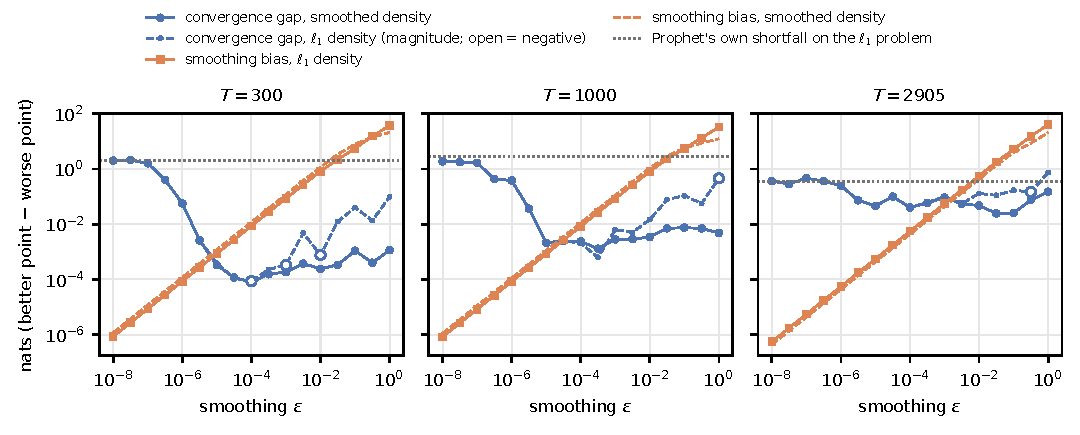
\includegraphics[width=\textwidth]{figures/smoothing}
  \caption{Prophet's Stan program with $\lvert\delta_j\rvert$ replaced by
    $\sqrt{\delta_j^2+\varepsilon^2}-\varepsilon$, fitted by Stan's own L-BFGS. Blue: the
    convergence gap, how far Stan stops short of the smoothed problem's own optimum.
    Orange: the smoothing bias, how far that optimum sits from Prophet's $\ell_1$ optimum.
    Solid lines are scored by the density each point was optimal for, dashed by the
    other; scored by Prophet's density the convergence gap is slightly negative in a few
    cells, drawn open at their magnitude. Dotted: Prophet's own shortfall on its actual
    problem. Peyton Manning, default configuration.}
  \label{fig:smoothing}
\end{figure}

At $\varepsilon = \SmoothEpsMin$ the smoothed program is Prophet's for every practical
purpose, and Stan stops short of its optimum by amounts comparable to Prophet's
shortfall on the $\ell_1$ problem: \SmoothGapAtMinShort, \SmoothGapAtMinMid{} and
\SmoothGapAtMinLong{} nats at the three lengths, against \LpMarginShort, \LpMarginMid{}
and \LpMarginLong. As $\varepsilon$
grows the convergence gap falls, by a factor of up to \SmoothDropShort, \SmoothDropMid{}
and \SmoothDropLong{} at the three lengths, while the smoothing bias rises, in proportion
to $\varepsilon$ up to $\varepsilon = 10^{-2}$, and the two cross near $\varepsilon = \SmoothCrossingShort$,
$\SmoothCrossingMid$ and $\SmoothCrossingLong$. At the best $\varepsilon$ on the grid
($\SmoothBestEpsShort$, $\SmoothBestEpsMid$ and $\SmoothBestEpsLong$), Stan's own L-BFGS on
the smoothed program lands within $\SmoothBestShort$, $\SmoothBestMid$ and
$\SmoothBestLong$ nats of Prophet's $\ell_1$ optimum --- \SmoothFactorShort, \SmoothFactorMid{}
and \SmoothFactorLong{} times closer than Prophet gets on its actual problem. Nothing but the
smoothness of the objective changed.

The gap does not vanish as $\varepsilon$ grows. Wherever $\varepsilon \ge 10^{-4}$ it
stays between $\SmoothPlateauMinShort$ and $\SmoothPlateauMaxShort$ nats at
$T = 300$, and between $\SmoothPlateauMinLong$ and $\SmoothPlateauMaxLong$ at $T = 2905$,
where Stan ends on its relative-gradient test, as it does in \SmoothStoppedGradient{} of
the \SmoothRuns{} runs. What remains there is not the kink, which the smoothed problem does
not have, but the point at which Stan's stopping rule declares a smooth problem
solved.

\paragraph{Outside Stan.}
The dependence on the kink is not peculiar to Stan's code. We ran SciPy's L-BFGS-B
\citep{byrd1995limited} with no bounds on the natural parameterisation, from Prophet's
initialisation and with its tolerances set to zero, at \StrengthLambdas{} values of
$\lambda = 1/\tau$ from $10^{-6}$ to $100$ at the three lengths. Here $\sigma$ is held at
Prophet's estimate, so that each problem is a quadratic plus
$\lambda\lVert\delta\rVert_1$ with a unique minimiser, which an active-set method
computes exactly; Stan's gradient certifies each with a relaxed residual of at most
$\StrengthReferenceResidual$. Wherever that minimiser has no rate at zero, L-BFGS
reaches it to within $\StrengthSmoothMax$ nats. As $\lambda$ grows and more of the
minimiser's rates sit on the kink, it stops further short: by \StrengthDefaultShort,
\StrengthDefaultMid{} and \StrengthDefaultLong{} nats at the default $\lambda = 20$,
where \StrengthDefaultZerosShort, \StrengthDefaultZerosMid{} and
\StrengthDefaultZerosLong{} of the 25 rates are zero. Across the \StrengthCells{} cells
the rank correlation between the shortfall and the number of zero rates is
\StrengthRankCorrelation.

\subsection{The solution path in $\tau$}
\label{sec:evidence:path}

With $\sigma$ fixed the problem is convex, and its minimiser moves continuously as $\tau$
changes --- piecewise linearly in $\lambda = 1/\tau$, as for the lasso
\citep{efron2004least}. With $\sigma$ free nothing guarantees it, but that is the setting
Prophet's users fit. We sweep $\lambda$ over \TauGlobalPoints{} values from \TauLamMin{}
to \TauLamMax{} on the Peyton Manning series in both settings. Prophet is refitted from
its own initialisation at every value, as a user changing \code{changepoint_prior_scale}
does; the exact path is computed by this implementation's Newton method on the
reformulation, warm-started from each neighbouring value and certified at every point,
with a relaxed residual of at most $\TauExactResidualMax$. Prophet's points sit a median
of \TauGapMedianFixed{} nats below the exact path with $\sigma$ fixed and
\TauGapMedianFree{} with it free, and up to \TauGapMax, with a median residual of
\TauProphetResidualMedian.

\begin{figure}[t]
  \centering
  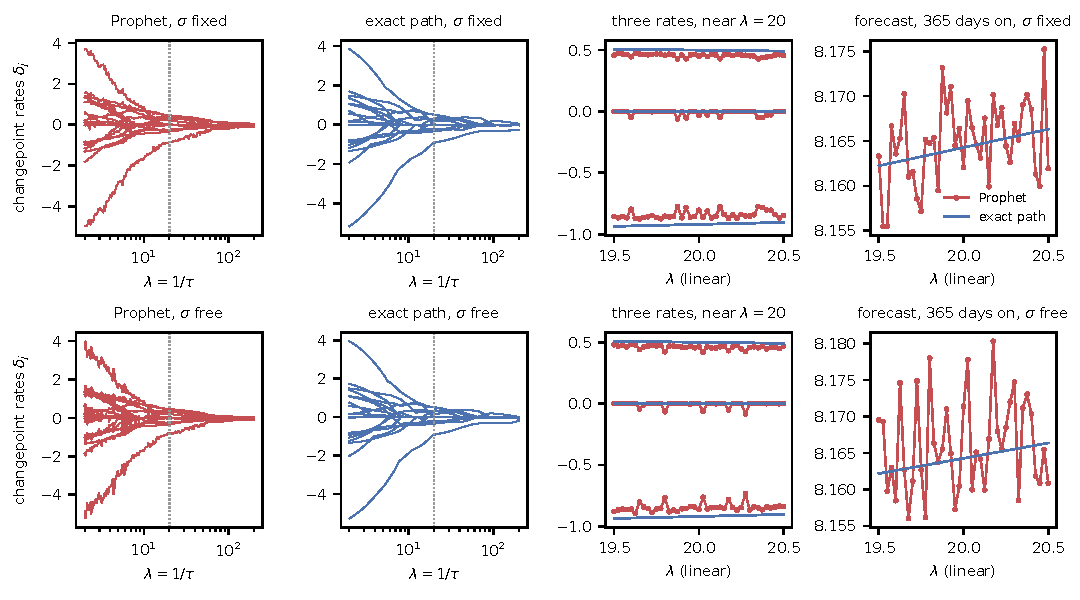
\includegraphics[width=\textwidth]{figures/tau_path}
  \caption{The solution path in $\lambda = 1/\tau$ on the Peyton Manning series. Left two
    columns: the 25 changepoint rates over the whole grid, Prophet's (Stan's L-BFGS from
    Prophet's initialisation at each $\lambda$) and the exact path. Right two columns:
    near the default $\lambda = 20$, on a grid \TauZoomStep{} apart, the three rates
    Prophet moves most and the forecast 365 days past the end of the series, both paths.
    Top row: $\sigma$ fixed, where the problem is convex; bottom row: $\sigma$ free.}
  \label{fig:tau}
\end{figure}

\Cref{fig:tau} shows a difference in kind. Near the default, on a grid \TauZoomStep{}
apart in $\lambda$, the exact path's rates move by a constant \TauExactZoomStep{} per
step, as a piecewise-linear path must, and Prophet's by as much as \TauProphetZoomMax{},
irregularly. Halving the interval of each path's largest step \TauLevels{} times, down to a
width of \TauFinalWidth{} in $\lambda$, separates steep motion from a jump: the exact
path's step halves every time, to $\TauExactFinal$, while Prophet's stays at
\TauProphetFinalFixed{} with $\sigma$ fixed and \TauProphetFinalFree{} with it free.
Prophet's path does not move steeply; it jumps, and the forecast jumps with it. This
implementation's default fit, from a cold start, stays within \TauDefaultDeviation{} of
the exact path.

\subsection{A negative control: removing the trend}
\label{sec:evidence:flat}

Under flat growth the likelihood never sees $k$ or $\delta$, so nothing pulls
against the prior and every changepoint rate goes to zero. Both implementations
then reach the same point: at each of the \FlatLengths{} lengths of
\cref{sec:evidence:lp} their $\lp$ agree to within $\FlatLpGap$ nats and their
parameters to within $\FlatParamGap$, and every one of the 25 rates is exactly zero
--- for Prophet as much as for this implementation.

This establishes that the two implementations fit the same model, so the margin
under linear growth is optimizer behaviour and not a difference of specification.
It does \emph{not} isolate the kink. Flat growth removes the ill-conditioned
$k$--$\delta$ directions and, at the same time, leaves the objective in $\delta$ as
$\tau^{-1}\sum_j\lvert\delta_j\rvert$ alone, a function every method minimises
exactly. The tie is consistent with either mechanism and the smoothing control of
\cref{sec:evidence:surrogate} is what separates them.

\subsection{One second-order method, two parameterisations}
\label{sec:evidence:newton}

To see what the kink costs a second-order method with everything else held fixed,
we run one damped Newton method on two parameterisations of the same objective. It
is this implementation's: a Hessian from central differences of the analytic
gradient, Levenberg damping, and Stan's stopping tests. On the natural
parameterisation the prior enters through its subgradient, with
$\operatorname{sign}(0) = 0$ as in Stan; on the reformulation of
\cref{sec:reformulation} it is linear. Both start from Prophet's own
initialisation, every rate at zero, on the Peyton Manning series at
\NewtonLengths{} lengths from $T = \NewtonLengthMin$ to $\NewtonLengthMax$. Only the
representation of $\delta$ differs.

On the reformulation the method reaches the optimum at every length, in
\NewtonSplitIterMin{} to \NewtonSplitIterMax{} iterations, with between
\NewtonSplitZerosMin{} and \NewtonSplitZerosMax{} of the 25 rates exactly zero. On
the natural parameterisation the same code oscillates: the rates change sign
between \NewtonFlipsMin{} and \NewtonFlipsMax{} times in a run, the progress of the
last hundred iterations falls to a median of $\NewtonProgressMin$ to
$\NewtonProgressMax$ nats a step, and Stan's stopping tests then declare
convergence, after \NewtonIterMin{} to \NewtonIterMax{} iterations, between
\NewtonShortMin{} and \NewtonShortMax{} nats short of the optimum and with no rate
exactly zero. It does not exhaust Prophet's budget of 10\,000 iterations; it stops
early and reports success.

Stan's own Newton is a different method, and it comes closer. Its Hessian is a
four-point finite difference of the gradient with a step of $10^{-3}$, wide enough
to straddle the kink wherever $\lvert\delta_j\rvert < 2\times10^{-3}$, and it damps by
reflecting negative eigenvalues rather than by adding to the diagonal. Run by
Prophet on the same series, it stops between \NewtonStanMin{} and \NewtonStanMax{}
nats short of the optimum: closer than the natural-parameterisation Newton at every
length, and at no length at the optimum, with no rate exactly zero.
